\chapter{SISTEMA DE COLAS SIMPLES}

\section{INTRODUCCIÓN}\label{intro}
En este capítulo se presenta el principal modelo de colas simples. En capítulos posteriores se
discutirán las redes de colas que son la extensión del modelo simple aquí estudiado. El modelo de
colas simple es el ladrillo a partir del cual se construye el edificio de la planeación de redes y el
análisis de desempeño en los sistemas de telecomunicaciones. La mayoría de trabajos de modelado
que se han hecho para sistemas de colas involucra, necesariamente, al menos una cola simple. La
principal razón es que para cualquier investigación en la teoría de colas, el sistema de cola simple es
un punto de partida natural. Otra razón es la facilidad de su tratamiento: Es mucho más fácil
formalizar los resultados con una cola simple para luego extenderlo a modelos más complejos de
red de colas.
\\
En particular, aquí se estudian los fundamentos del sistema de colas básico, llamado $( M/M/1)$: Este es un modelo de colas “Markoviano” en el que se distingue un proceso de llegada de Poisson y
tiempo de servicio exponencial. Para representar la dinámica de ese sistema se emplean los
diagramas de transición de estados.


\section{EXPRESIÓN DE KENDALL Y MEDIDAS DE DESEMPEÑO.}\label{intro}
\subsection{Notación.}
Para referirse formalmente a los principales elementos matemáticos que hacen parte de un sistema
de líneas de espera (o colas) es ampliamente aceptada la notación de seis (6) parámetros propuesta
por Kendall. En dicha convención se expresa un sistema de líneas de espera mediante el siguiente formato de la expresión \ref{eqn:1.1}.

\begin{equation}
    \left( a/b/c \right) :\left( d/e/f \right)
    \label{eqn:1.1}
\end{equation}
\\
Cada uno de los tres parámetros que conforman las dos secciones presentes en la expresión \ref{eqn:1.1}
tienen un significado asociado. En la primera sección, el parámetro {\em a} representa la estructura (o familia) probabilística que guía la llegada de clientes al sistema; el parámetro {\em b} se emplea para
indicar la estructura probabilística del tiempo de atención por parte del servidor o de los servidores.
Ellos usualmente se sustituyen por las letras mayúsculas {\em M} que indica {\em “Markoviano”} y que implica que el número de clientes corresponde a un proceso de {\em Poisson}; la letra
{\em D} significa {\em “determinístico”} o {\em “degenerado”} queriendo decir que los tiempos de llegada (o atención según el caso) son constantes y no variables aleatorias. La letra {\em G} se utiliza para indicar que la familia probabilística es {\em “general”} es decir cualquiera. Por su lado, el último parámetro de la primera sección, \(c \in \mathbb{N}\)
, es una constante natural que indica el número de servidores en paralelo que trabajan
en el sistema (usualmente $ c = 1 $).
\\
Los parámetros de la segunda sección de la referida expresión también tienen sus significados
específicos. El parámetro {\em d} se emplea para indicar la disciplina de servicio; esto es, el mecanismo
que empleará el servidor para seleccionar al siguiente cliente que él va a atender una vez se
desocupe del cliente que está actualmente atendiendo. Este parámetro es frecuentemente FIFO
(primero en llegar primero en ser atendido); sin embargo, hay otras opciones. Por ejemplo LIFO
(último en llegar, primero en ser atendido). Por su parte, el parámetro $ c \in \mathbb{N} $ representa la capacidad del sistema; es decir, el número máximo de clientes (simultáneos) que pueden permanecer dentro del
sistema. Finalmente, el tamaño de la población, origen de los clientes, lo representa el parámetro {\em f}.
\\
\\
\textbf{Ejemplo 1—1: Un sistema de líneas de espera.}

La expresión (Cauchy$(\alpha,\beta )$/Uniforme$( \eta ,\mu  )$/7):(LIFO/180/1.000.000) describe un sistema de líneas de espera con tiempos entre llegadas de la familia Cauchy, tiempo de atención en los 7 servidores en paralelo de la familia uniforme. Política de atención LIFO, máximo 180 clientes dentro del sistema (capacidad de la fila 180-7=173) y tamaño de la población de donde provienen los clientes de un millón.
\\
\textbf{\textit{Observación:}}
Cuando en esta nomenclatura se suprime la segunda sección se supone: Política FIFO, Capacidad
del sistema y tamaño de la población infinitos. Esquemáticamente eso significa:
\begin{equation}
    \left ( a/b/c \right ) = \left ( a/b/c \right ) : \left ( FIFO/+\infty/+\infty\right )
    \label{eqn:1.2}
\end{equation}

\subsection{Medidas de desempeño.}
Especificar el sistema no es suficiente. A partir de esa especificación formal se deben obtener medidas que describan de alguna manera el comportamiento o desempeño de ese sistema. Aunque esas medidas de desempeño pueden ser de diferentes formas y de distintas propiedades, es frecuente intentar calcular: (1) El número medio de clientes en el sistema, (2) El número de clientes esperado en fina, (3) El tiempo promedio dentro del sistema, (4) El tiempo medio de permanencia en cola
(fila) y (5) La utilización, que se define como el porcentaje de tiempo que los servidores permanecen ocupados. Aquí solo nombramos cinco pero la lista puede crecer tanto como se quiera.

\begin{figure}[H]
\centering
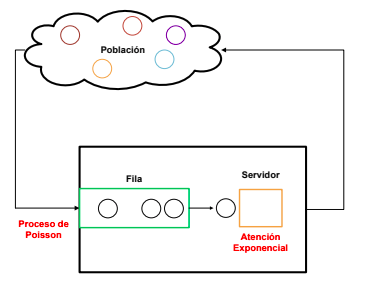
\includegraphics[width=3in]{chapters/chapter3/figures/Figura1-1:Sistema(mm1).png}
%%\centerline{\epsfig{/Chapters/chapter3/figures/Figura1-1:Sistema(mm1).png,width=.8\textheight,height=.4\textwidth}}
\caption[Sistema (M/M/1)]{Sistema (M/M/1)}
\label{fig:mesh1}
\end{figure}

\section{SISTEMA DE COLAS \textit{(M/M/1)}}
Considérese el sistema de la Figura \ref{fig:mesh1}. Ese es el sistema de colas simple del cual parte la teoría de colas. El sistema $(M/M/1)$ tiene dos supuestos importantes. El primero es que el proceso de llegadas es un proceso de Poisson, y el otro que cuenta con un único servidor razón por la cual tiene un único tiempo de servicio que corresponde a una variable con distribución exponencial. Estos supuestos llevan a un modelo muy manejable y además razonable, para una gran variedad de situaciones. Se examinarán ahora estos dos supuestos.
\subsection {Procesos binomiales y Procesos de Poisson.}
El $proceso$ $de$ $Poisson$ es el proceso de llegada más sencillo. Una forma de entenderlo es esta. Suponga que el eje temporal se divide en un gran número de pequeños segmentos de longitud
$ \Delta t $. Se supone que la probabilidad de que un único cliente llegue a un segmento es proporcional a la
longitud de ese segmento,$ \Delta t $, multiplicado por una constante de proporcionalidad, multiplicado por una constante de proporcionalidad, $ \lambda $, que representa la tasa media de llegadas:
\begin{equation}
    P\left [ Exactamente \; 1 \; llegada \;en \left [ t,t+\Delta t \right ] \right ] = \lambda \Delta t
    \label{eqn:1.3}
\end{equation}

\begin{equation}
    P\left [ No \;llega \;en  \left [ t,t+\Delta t \right ] \right ] = 1-\lambda \Delta t
    \label{eqn:1.4}
\end{equation}

\begin{equation}
    P\left [ M\acute{a}s\; de \; 1 \; llegada\; en  \left [ t,t+\Delta t \right ] \right ] = 0
    \label{eqn:1.5}
\end{equation}
\\
Aquí (dada su magnitud) se ignoran los términos de orden superior que involucren $ \Delta t $. Es posible hacer una analogía entre el proceso de llegada y el lanzamiento de una moneda en cada uno de los segmentos. Aquí la probabilidad de llegada es $ \lambda \Delta t $ (es decir, cara) y $1-\lambda \Delta t$ es la probabilidad de
no llegada (es decir, sello). Los lanzamientos, y en consecuencia los resultados, de cada moneda son, a simple vista, independientes unos con otros; por esta razón, al observar el comportamiento del sistema en un intervalo de tiempo $\left [ 0,t \right )$ en el cual se pueda escribir $t = n\Delta t $ con $ c \in \mathbb{N} $ y, en consecuencia, $ t \in \mathbb{R}^{+} $ , es claro que al definir la variable aleatoria $ N_{t} $ como el número de clientes que arriban al sistema en $ \left [ 0,t \right ) $ su estructura probabilística es $ N_{t} \sim Binomial \left ( n,p=\lambda \Delta t \right ) $ o, más específicamente, $ f_{N_{t}}\left ( k;n,p=\lambda \Delta t \right ) = P \left [ N_{t} = k \right ] $ , está dada en la ecuación \ref{eqn:1.6}.

\begin{equation}
    f_{N_{t}}\left ( k;n,p=\lambda \Delta t \right ) = \binom{n}{k}\left ( \lambda \Delta t \right )^{k}\left ( 1 - \lambda \Delta t \right )^{1-k}
    \label{eqn:1.6}
\end{equation}
\\
De ahí que la estructura probabilística dependa del tiempo de observación del sistema $ t $ y que, por lo tanto, rigurosamente hablando, a este modelo se le conozca con el nombre de \textit{Procesos estocásticos binomiales de nacimiento puro}. Cuando $ \Delta t \rightarrow 0 $ se obtiene un proceso de Poisson de tiempo continúo puesto que, como se mostrará más adelante, una familia binomial converge a una familia de Poisson cuando $ n \rightarrow 0 $, $ p=\lambda \Delta t  \rightarrow 0 $ y $ \mu _{N_{t}}= p \times n = \lambda $  permanece constante. En este escenario, cada lanzamiento de una moneda puede ser una analogía de las llegadas, unas independientes de otras, ya que se puede pensar en un simple resultado positivo de una larga lista de lanzamientos de monedas independientes. Además, se puede ver todos los intervalos de tiempo tienen la misma probabilidad constante de tener una llegada.


\begin{figure}[H]
\centering
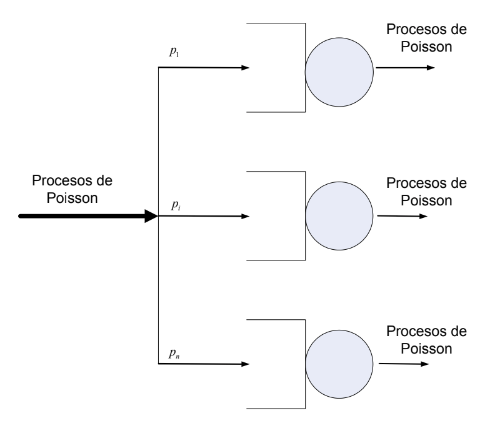
\includegraphics[width=3in]{chapters/chapter3/figures/Figura1-2:BifurcaciondeunprocesodePoisson.png}
%%\centerline{\epsfig{/Chapters/chapter3/figures/Figura1-1:Sistema(mm1).png,width=.8\textheight,height=.4\textwidth}}
\caption[Bifurcación de un proceso de Poisson]{Bifurcación de un proceso de Poisson}
\label{fig:mesh2}
\end{figure}

\subsection{Dos propiedades importantes de los procesos de Poisson.}
Dos ideas importantes caracterizan a los procesos de Poisson. La primera es el proceso de bifurcación aleatoria de un proceso de Poisson y la segunda es la unión de varios procesos de Poisson. La Figura \ref{fig:mesh2} ilustra un sistema de filas con variables ramificación o bifurcaciones. La llegada se divide aleatoriamente entre $ n $ ramas con probabilidades independientes $ p_{1},\cdots,p_{i},\cdots, p_{n} $. La segunda, que se ilustra en la Figura \ref{fig:mesh3}, es una situación que envuelve la unión de procesos de Poisson independientes. En este caso, las llegadas de un número de procesos independientes se unen o fusionan en un único proceso agregado.
Una de las aplicaciones originales, aunque no la única ni la más importante, de los procesos de Poisson en redes de comunicaciones es el modelo de llegadas de llamadas a una central telefónica. 

El uso de cada teléfono, por lo menos en un primer análisis, puede ser modelado por un proceso de Poisson. Así, modelar puede convertirse en algo complicado, pero es indudable la elegancia de formular este tipo de modelos para realizar planeación de redes de computadores y de telecomunicaciones de una manera formal y bella. El punto importante está en que tanto los procesos de ramificaciones aleatorias como las uniones de procesos de Poisson resultan ser también Procesos de Poisson. La analogía del lanzamiento de monedas sirve para demostrar de una manera muy sencilla que estos resultados son verdad.

\begin{figure}[H]
\centering
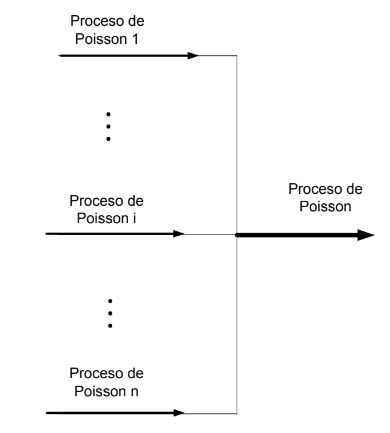
\includegraphics[width=2in]{chapters/chapter3/figures/Figura1-3:UniondeVariosprocesosdePoisson.png}
%%\centerline{\epsfig{/Chapters/chapter3/figures/Figura1-1:Sistema(mm1).png,width=.8\textheight,height=.4\textwidth}}
\caption[Unión de varios procesos de Poisson]{Unión de varios procesos de Poisson}
\label{fig:mesh3}
\end{figure}

\subsection{Fundamentos del proceso de Poisson.}
En este apartado se deduce una ecuación diferencial que se obtiene del proceso de Poisson a partir del modelo discreto resulta de partir de pequeños intervalos $ \Delta t $ de tiempo para, finalmente, tomar
el límite cuando $ \Delta t \rightarrow 0 $. En primer lugar

\begin{equation}
    P_{n}\left ( t \right ) = P \left ( \#\; llegan = n\; en\; tiempo\; t \right )
    \label{eqn:1.7}
\end{equation}
\\
Además, sea $ P_{ij}\left (  \Delta t \right ) $ la probabilidad de pasar de $i$ llegadas (nacimientos) a $j$ en $ \Delta t$ segundos.El proceso de deducción que aquí se presenta está inspirado en el libro \cite{kleinrock1975}. En este modelo, el número de llegadas (o nacimientos) es el “estado” del sistema. Este dato contiene toda la información necesaria para describir el sistema de una manera adecuada. Dicho esto, es claro, entonces que para esta situación se cumple la ecuación \ref{eqn:1.8}

\begin{equation}
    P_{n}\left ( t + \Delta t \right ) = P_{n}\left ( t \right )P_{n,n}\left ( \Delta t \right )+P_{n-1}\left ( t \right )P_{n-1,n}\left ( \Delta t \right )
    \label{eqn:1.8}
\end{equation}
\\
Nuevamente aquí, no se tiene en cuenta (por ser de magnitudes muy pequeñas) los términos de orden superior en $ \Delta t $. Lo que dice la ecuación \ref{eqn:1.8} es que el sistema puede llegar al estado $n$, esto tener clientes o nacimiento en el tiempo en el intervalo $ \left [ 0,t + \Delta t \right ) $ ya sea porque en el intervalo $ \left [ 0,t \right ) $ el sistema ya se encontraba en el estado $ n $ y que durante el intervalo $ \left [ t,t + \Delta t \right ) $ no haya habido ninguna llegada, o bien, que en el intervalo $ \left [ 0,t \right ) $ el sistema estaba en el estado
$ n-1 $ y que durante el intervalo $ \left [ t,t + \Delta t \right ) $ haya habido una llegada. Nótese que se puede asumir que $ \Delta t $ es suficientemente pequeño de modo que es razonable suponer que a lo sumo un cliente puede llegar durante este intervalo. 


\begin{figure}[H]
\centering
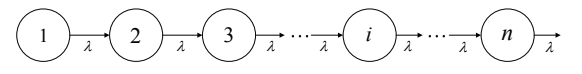
\includegraphics[width=3in]{chapters/chapter3/figures/Figura1-4:DiagramadetransiciondeestadosdeunprocesodePoisson.png}
\caption[Diagrama de transición de estados de un proceso de Poisson]{Diagrama de transición de estados de un proceso de Poisson}
\label{fig:mesh4}
\end{figure}

Para este sistema, el diagrama de transición de estados se presenta en la Figura \ref{fig:mesh4} 1—4, en él los
círculos representan los estados del sistema (número de llegadas o nacimientos) y $ \lambda $ representa la
razón (clientes por unidad de tiempo) asociada con cada transición. Adicionalmente, se necesita la condición de frontera, es decir la probabilidad para el estado $ n = 0 $, cuya expresión se muestra en la ecuación \ref{eqn:1.9}
\\
\begin{equation}
    P_{0}\left ( t+ \Delta t \right )=P_{0}\left ( t \right )P_{0,0}\left ( \Delta t \right )
    \label{eqn:1.9}
\end{equation}
\\
Las expresiones \ref{eqn:1.8} y \ref{eqn:1.9} son suficientes para determinar completamente $ P_{n} \left ( t \right ) $. Al sustituir las probabilidades de las expresiones \ref{eqn:1.3}, \ref{eqn:1.4} y \ref{eqn:1.5} en las ecuaciones \ref{eqn:1.8} y \ref{eqn:1.9} se obtiene \ref{eqn:1.10}.

\begin{equation}
    P_{n}\left ( t+\Delta t \right )=P_{n}\left ( t \right )\left ( 1-\lambda \Delta t \right )+P_{n-1}\left ( t \right )\left ( \lambda \Delta t \right )
    \label{eqn:1.10}
\end{equation}
\\
A partir de \ref{eqn:1.10} y aplicando algunas operaciones elementales y reorganizando se llega a \ref{eqn:1.11}.

\begin{equation}
    \frac{P_{n}\left ( t+\Delta t \right ) - P_{n}\left ( t \right ) }{\Delta t}=-\lambda P_{n}\left ( t \right )+\lambda P_{n-1}\left ( t \right )    
    \label{eqn:1.11}
\end{equation}
\\
Y de forma similar a partir de \ref{eqn:1.9} se llega a \ref{eqn:1.12} 

\begin{equation}
    \frac{P_{0}\left ( t+\Delta t \right ) - P_{0}\left ( t \right ) }{\Delta t}=-\lambda P_{0}\left ( t \right )
    \label{eqn:1.12}
\end{equation}
\\
Al tomar el límite cuando, en \ref{eqn:1.11} y \ref{eqn:1.12}, $ \Delta t \rightarrow 0 $ , este conjunto de ecuaciones se obtiene \ref{eqn:1.13}. En ella $ n\geq 1 $, y se desea, naturalmente, encontrar la solución a estas ecuaciones diferenciales,$ P_{n}\left ( t \right ) $.

\begin{equation}
    \frac{d P_{n}\left ( t \right )}{dt} = -\lambda P_{n}\left ( t \right )+\lambda P_{n-1}\left ( t \right )
    \label{eqn:1.13}
\end{equation}
\\
y 

\begin{equation}
    \frac{dP_{0}\left ( t \right )}{dt} = -\lambda P_{0}\left ( t \right )
    \label{eqn:1.14}
\end{equation}
\\
De la ecuación \ref{eqn:1.14}, es trivial, observar que su solución es \ref{eqn:1.15}

\begin{equation}
    P_{0}\left ( t \right )=e^{-\lambda t}
    \label{eqn:1.15}
\end{equation}
\\
Para $ n = 1 $ se parte de la ecuación \ref{eqn:1.13} en la cual se reemplaza el resultado \ref{eqn:1.15} con lo cual se llega a la ecuación diferencial \ref{eqn:1.16}.

\begin{equation}
    \frac{dP_{1}\left ( t \right )}{dt} = -\lambda P_{1}\left ( t \right )+\lambda e^{-\lambda t}
    \label{eqn:1.16}
\end{equation}
\\
La solución de la ecuación diferencial \ref{eqn:1.16} esta dada en \ref{eqn:1.17}.

\begin{equation}
    P_{1}\left ( t \right )=\lambda te^{-\lambda t}
    \label{eqn:1.17}
\end{equation}
\\
De forma similar la siguiente ecuación diferencial, con $ n = 2 $, es \ref{eqn:1.18}.

\begin{equation}
    \frac{dP_{2}\left ( t \right )}{dt} = - \lambda P_{2}\left ( t \right ) + \lambda^{2}te^{-\lambda t}
    \label{eqn:1.18}
\end{equation}
\\
Por su parte, la solución de \ref{eqn:1.18} es \ref{eqn:1.19}.

\begin{equation}
    P_{2}\left ( t \right )=\frac{\Delta ^{2}t^{2} }{2} e^{-\lambda t}
    \label{eqn:1.19}
\end{equation}
\\
Continuando con un proceso idéntico, se puede encontrar por inducción matemática que la solución general de la ecuación diferencial dada en \ref{eqn:1.13} es la función \ref{eqn:1.20}.

\begin{equation}
    P_{n}\left ( t \right )=\frac{ \left ( \lambda t  \right )^{n} }{n!} e^{-\lambda t}
    \label{eqn:1.20}
\end{equation}
\\
Esta es, como puede notarse por simple inspección, que \ref{eqn:1.20} es la  {\em distribución de Poisson}. En este caso modela la probabilidad de $n$ llegadas (nacimientos) en un intervalo de $n$ segundos para un proceso de Poisson de parámetro $ \lambda $.
\\
\textbf{Ejemplo 1—2: Proceso de Poisson.}
\\
Una central telefónica recibe en promedio 100 llamadas por minuto, de acuerdo con un proceso de Poisson. ¿Cuál es la probabilidad de que no entren llamadas en un intervalo de 5 segundos?
\\\\
La solución es simple. $P_{0}\left ( \frac{1}{12} \right )=e^{-\lambda t}=e^{100*\frac{1}{12}}=0.00024$

\subsection{Media y varianza de un proceso de Poisson.}
Ahora se hará la deducción de la media Ahora se hará la deducción de la $media$ $\mu _{t}$ y la varianza $\sigma _{t}^{2}$ de una distribución de $Poisson.$
Sea $\mu _{t}$ el número medio de llegadas en un intervalo de longitud $t$. De esta manera los cálculos presentados en \ref{eqn:1.21} son los primeros pasos para obtener el resultado. La primera igualdad corresponde a la definición, en la segunda se emplea la expresión \ref{eqn:1.20} mientras que en la tercera y última serie de igualdades se factorizan aquellos elementos que no dependen del índice de la sumatoria.

\begin{equation}
    \mu_{t}=E\left [ N_{t} \right ]=\sum_{n=0}^{\infty}n\left [ \frac{\left ( \lambda t \right )^{n}}{n!}e^{-\lambda t} \right ]=e^{-\lambda t}\sum_{n=1}^{\infty}n\frac{\left ( \lambda t \right )^{n}}{\left ( n-1 \right )!}
    \label{eqn:1.21}
\end{equation}
\\
La deducción continúa en \ref{eqn:1.22} con un cambio de variable muy simple, $ m = n-1 $, y luego, nuevamente, factorizando elementos que no son funcionalmente dependientes del índice de la sumatoria y, finalmente, recordando la expansión en series de Taylor de la función exponencial.

\begin{equation}
    \mu_{t}= e^{-\lambda t}\sum_{m=0}^{\infty}n\frac{\left ( \lambda t \right )^{m+1}}{m!}=e^{-\lambda t} \lambda t \sum_{m=0}^{\infty}n\frac{\left ( \lambda t \right )^{m}}{m!}=e^{-\lambda t}\lambda t\left ( e^{\lambda t} \right )=\lambda t
    \label{eqn:1.22}
\end{equation}
\\
La ecuación $ \mu_{t}=\lambda t $ es un resultado muy intuitivo y, por la misma razón, muy bella. Ella indica que el número medio $ \mu _{t} $ es proporcional a la longitud del intervalo $ t $ y a la razón de llegadas de clientes por unidad de tiempo $ \lambda $. Por su parte, para la varianza $\sigma _{t}^{2}$ , el tratamiento adoptado en este texto es similar al presentado en \cite{kleinrock1975}. Sin embargo, antes de entrar de lleno en su deducción, es útil calcular la siguiente esperanza matemática que aplica para un proceso de Poisson. 

\begin{equation}
    E\left [ N_{t}\left ( N_{t}-1 \right ) \right ]=\sum_{n=0}^{\infty}n\left ( n-1 \right )\frac{\left ( \lambda t \right )^{n}}{n!}e-\lambda t = \sum_{n=2}^{\infty}\frac{\left ( \lambda t \right )^{n}}{\left ( n-2 \right )!}e^{- \lambda t}
    \label{eqn:1.23}
\end{equation}
\\
Ahora, haciendo el cambio de variable $ m=n-2 $ y luego recordando la expansión en series de Taylor para la función exponencial se obtiene \ref{eqn:1.24}.

\begin{equation}
    E\left [ N_{t}\left ( N_{t}-1 \right ) \right ]=e^{- \lambda t}\left ( \lambda t \right )^{2} \sum_{m=0}^{\infty}\frac{\left ( \lambda t \right )^{m}}{m!}=\left ( \lambda t \right )^{2}
    \label{eqn:1.24}
\end{equation}
\\
Con este resultado es fácil deducir la variabilidad en un proceso de Poisson. En primer lugar, la identidad de la varianza \ref{eqn:1.25} brinda un camino.

\begin{equation}
    \sigma _{t}^{2}=E\left [ N_{t}^{2} \right ]-\mu _{t}^{2}
    \label{eqn:1.25}
\end{equation}
\\
Obsérvese que basta con calcular $ E\left [ N_{t}^{2} \right ] $ puesto que $ \mu _{t}^{2}=\left ( \lambda t \right )^{2}  $ como consecuencia de \ref{eqn:1.22}.
Ahora bien, este dato faltante puede encontrarse como se indica en \ref{eqn:1.26}. Ahí se aplican los resultados obtenidos en \ref{eqn:1.22} y \ref{eqn:1.24}.

\begin{equation}
    E\left [ N_{t}^{2} \right ]=E\left [ N_{t} \right ]+E\left [ N_{t} \left (  N_{t}-1 \right )\right ]=\left ( \lambda t \right )^{2}+\lambda t 
    \label{eqn:1.26}
\end{equation}
\\
Sustituyendo \ref{eqn:1.26} y \ref{eqn:1.22} en \ref{eqn:1.25} se concluye \ref{eqn:1.27}, es decir la varianza del proceso.

\begin{equation}
    \sigma _{n}^{2}=\left ( \lambda t \right )^{2}+\lambda t-\left ( \lambda t \right )^{2}=\lambda t
    \label{eqn:1.27}
\end{equation}
\\
En síntesis, el número medio de clientes y su varianza en un proceso de Poisson de nacimientos puros son, respectivamente, $ \mu _{t}=\lambda t $ y $ \sigma _{n}^{2}=\lambda t $.

\subsection{Tiempo entre llegadas.}
El tiempo entre eventos sucesivos en un proceso de llegada (o nacimiento puro) se denomina $tiempo$ $inter$-$llegadas$ o $tiempo$ $entre$ $llegadas$. Para un proceso de Poisson (de nacimiento puro), esos
tiempos son variables aleatorias independientes, distribuidas exponencialmente. Para ver que esto es verdad, sea $T$ el tiempo que trascurre entre dos llegadas sucesivas en un proceso de Poisson, la distribución de $T$ , esto es $F_{r}\left ( t \right )$ ,luego de unos breves pasos, es la expresión dada en \ref{eqn:1.28}.

\begin{equation}
    F_{r}\left ( t \right )=P\left [ T\leq t \right ]=1-P\left [ T>t \right ]=1-P_{0}(t)=1-e^{-\lambda t}
    \label{eqn:1.28}
\end{equation}
\\
Al derivar \ref{eqn:1.28} se encuentra  $f_{r}\left ( t \right )$ , la función de densidad de $T$ ,ésta función se muestra en \ref{eqn:1.29}.
\begin{equation}
    f_{T}\left ( t \right )=\lambda e^{-\lambda t }
    \label{eqn:1.29}
\end{equation}
\\
La expresión \ref{eqn:1.29} es la estructura probabilística del tiempo entre llegadas $T$ y, claramente, pertenece a la $familia$ {\em paramétrica} $exponencial.$

\subsection{Propiedad de pérdida de la memoria.}
La familia exponencial, es la única variable aleatoria continua que tiene la $propiedad$ $de$ {\em pérdida} $de$ $memoria.$ El concepto se puede entender con un ejemplo sencillo. Suponga que un tren llega a una estación de acuerdo con un proceso de Poisson con tiempo medio entre trenes de 20 minutos.
\\\\
Supóngase ahora que un pasajero llegada a la estación y que alguien que está esperando en la plataforma le informa que el último tren llegó hace 19 minutos. ¿Cuál es el tiempo medio que el pasajero que recién llega a la estación de be esperar antes de que el próximo tren llegue?
\\\\
El sentido común (el cual no siempre es un buen consejero) diría que la respuesta natural es un minuto, y esto sería verdad en el caso en el cual la llegada del tren fuera un evento determinístico separado exactamente por veinte minutos. Sin embargo, como se trata de un proceso de llegadas de
Poisson, ¡La respuesta es 20 minutos!
\\\\
Intuitivamente, la explicación de ello es sencilla. Para ver que esto es verdad, es necesario volver atrás con la explicación de lanzamiento de monedas del proceso de Poisson. Una llegada es un evento con resultado positivo (“éxito”) de un “lanzamiento de monedas” en un intervalo infinitamente pequeño. A medida que el tiempo avanza es como un gran número de lanzamientos de monedas. Cuando se pone el proceso de Poisson en este contexto es fácil ver que la distribución hasta el próximo evento positivo, esto es “éxito”, no depende de cuando tiempo ha pasado desde el último evento positivo.
\\\\
Sin embargo, el razonamiento intuitivo no es suficiente. La deducción formal o matemática, es decir, ya no intuitiva, es importante y se encuentra de la siguiente manera. Supóngase que una llegada ocurre en el tiempo $t$=0, se sabe, además de \ref{eqn:1.29}, que la estructura probabilística del
tiempo antes de la siguiente llegada, $T$ , es exponencial. También supóngase ahora que no han ocurrido llegadas antes del tiempo $t_{0}$.
Dada esta información, se desea responder la pregunta ¿cuál
es la distribución del tiempo antes de la siguiente llegada? La respuesta se deduce aquí de forma similar a la expuesta en [1] con la definición de una variable aleatoria ficticia $T^{*}$ y, con ella, deducir su función de distribución $F_{T^{*}}\left ( t \right )$.
\\\\
Por definición de función de distribución $F_{T^{*}}\left ( t \right )=P\left [ T^{*}\leq t \right ]$ e incorporando la información disponible
$F_{T^{*}}\left ( t \right )=P\left [ T^{*}\leq t_{0}+t|T^{*}>t_{0} \right]$. 
\\
Ahora, teniendo en cuenta la definición de probabilidad condicional

$F_{T^{*}}\left ( t \right )=\frac {P\left [ T^{*}\leq t_{0}+t,\wedge ,T^{*}>t_{0} \right ]} {P\left[T^{*}>t_{0}\right ]}=\frac{P\left [ t_{0}<T^{*}\leq t+t_{0} \right ]}{P\left [ T^{*}>t_{0} \right ]}$. De acuerdo con las propiedades de la función de distribución y teniendo en cuenta la expresión \ref{eqn:1.28} 
\\
$F_{T^{*}} \left ( t \right )=\frac {F_{T^{*}}\left ( t+t_{0} \right )-F_{T^{*}}\left ( t_{0} \right )}  {1-F_{T^{*}}\left ( t_{0} \right )}=\frac {\left ( 1-e^{-\lambda \left ( t+t_{0} \right )} \right )-\left ( 1-e^{-\lambda t_{0}} \right )}   {1-\left ( 1-e^{-\lambda t_{0}} \right )}$ de donde se deduce \ref{eqn:1.30}.
\\

\begin{equation}
    F_{T^{*}}\left ( t \right )=1-e^{-\lambda t}
    \label{eqn:1.30}
\end{equation}
\\
Lo que, en palabras sencillas, significa que la estructura probabilística de $T^{*}$ , el tiempo que se debe esperar hasta la siguiente llegada dado que se sabe que ese tiempo $T^{*}$ es más grande que $t^{_{0}}$ , es una variable aleatoria perteneciente a la familia exponencial. Ello implica que $\mu _{T^{*}}=\frac{1}{\lambda }$ y que $\sigma _{T^{*}}^{2}=\frac{1}{\lambda ^{2}}$.
\\\\
Se termina este apartado señalando que la familia paramétrica $discreta$ con la propiedad de pérdida de memoria es la distribución {\em geométrica} razón por la cual se dice que la familia exponencial es al mundo continuo lo que la familia geométrica al mundo discreto. Ambas familias juegan un papel protagónico en los modelos de tráfico en redes de telecomunicaciones.






\subsection{La propiedad de Markov.}
La propiedad de pérdida de memoria se define con mayor precisión como la $propiedad$ $de$ $Markov$. Esta propiedad establece que es posible predecir un estado futuro de un sistema basado (únicamente) en el estado sin necesidad de conocer completamente su historial pasado. En términos de una variable aleatoria real no negativa $ T\in\mathbb{R}^{+}T $, la propiedad de Markov se formaliza, de acuerdo con \cite{kleinrock1975}, en la expresión \ref{eqn:1.31}, para un $t_{0}>0$ dado y específico y para cada $t>0$.

\begin{equation}
    P\left [ T>t_{0}+t|T>t_{0} \right ]=P\left [ T>t \right ]
    \label{eqn:1.31}
\end{equation}
\\
En términos de una variable aleatoria discreta X$\left ( t_{n} \right )$ , la misma propiedad se puede escribir, de acuerdo con [1], como en la expresión \ref{eqn:1.32}. Ahí, los  $t_{i}$ crecen monótonamente y los valores $x_{n}$ pertenecen a un espacio de estados discretos.

\begin{eqnarray}
   P\left [ X\left ( t_{n+1} \right )=x_{n+1}|X\left ( t_{n} \right )=x_{n},\cdots ,X\left ( t_{1} \right )=x_{1} \right ]= \nonumber \\
   P\left [ X\left ( t_{n+1} \right )=x_{n+1}|X\left ( t_{n} \right )=x_{n} \right ]
    \label{eqn:1.32}
\end{eqnarray}
\\
%\begin{eqnarray*}
% \lefteqn{ \sin z = z - \frac{z^3}{3!} +} \\
% & & + \frac{z^5}{5!} - \frac{z^7}{7!} + \cdots
%\end{eqnarray*}
Los sistemas Markovianos son sistemas con pérdida de la memoria. Esto hace que sea “muy simple” su análisis teórico puesto que resulta relativamente fácil describir los cambios de estado del sistema, uno necesita tener en cuenta el tiempo desde la última llegada, o el tiempo que el servicio
ha estado en curso desde el último cliente. Cuando el servicio no es Poisson, lo que significa que no se cuenta con la propiedad de pérdida de la memoria, o el tiempo de servicio no es exponencial entonces no se cuenta con las premisas necesarias para aprovechar ésta virtud. En este caso, el análisis del sistema, incluso en una cola simple, no es un trabajo trivial.
\\\\
Un concepto estrechamente relacionado con la propiedad markoviana es el de $cadena$ $de$ $Markov$. Una cadena de Markov es un proceso (estocástico) de Markov, con un espacio de estados discreto. La Figura 1—4, muestra un diagrama de transición de estados, $DTE$, del sistema de líneas de espera
$(M/M/1)$, en él se ilustra la sencillez que presume garantizar la propiedad de pérdida de la memoria para modelar su comportamiento.



\subsection{Tiempos de servicio exponencial.}
Una conclusión derivada de lo discutido en la sección 1.3.7 es que en un sistema $ \left ( M/M/1 \right ) $
el proceso de llegada, el proceso de llegada, representado por la primera $ M $, es “markoviano” lo que es equivalente a asegurar que (1) el número de clientes que llegan al sistema en un intervalo de tiempo de longitud $ t $ fijo es una variable aleatoria de Poisson, o bien que (2) el tiempo que trascurre entre la llegada del {\em (i-1)-ésimo } y es el {\em i-ésimo } clientes es una variable aleatoria exponencial $ T_{i}\sim Exp\left ( \lambda \right ) $ con independencia entre los $ T_{i} $'s. En consecuencia, se ha reiterado bastante, la estructura probabilística de los tiempos entre llegadas es $ f_{T}\left ( t \right )=\lambda e^{-\lambda t} $ y, por ello, el tiempo medio entre llegadas es $ \mu _{T}=\frac{1}{\lambda} $ mientras que la varianza del tiempo entre llegadas es $ \sigma _{T}^{2}=\frac{1}{\lambda^{2}} $. 
\\
\\
Por otro lado, la segunda $ M $ en un sistema $ \left ( M/M/1 \right ) $ indica que el tiempo $ S_{i} $ que el servidor emplea para atender al {\em i-ésimo } cliente también exhibe la propiedad markoviana; con todo lo que
ello implica. Por ejemplo, implica la propiedad de pérdida de la memoria y la independencia entre los tiempos que el servidor “gasta” atendiendo al cliente $ i $. También implica que los $ S_{i}\sim Exp\left ( \lambda \right ) $. En específico $ f_{S}\left ( s \right )=\mu e^{-\mu s} $ y, por ello, el tiempo medio de atención es $ \mu _{T}=\frac{1}{\mu} $ mientras que la varianza del tiempo de atención es $ \sigma _{S}^{2}=\frac{1}{\mu^{2}} $. En el caso de los tiempos de servicio como variables aleatorias exponenciales $ \mu $ es la tasa de atención (clientes por unidad de tiempo) mientras que $ \frac{1}{\mu} $ es la media del tiempo servicio (unidades de tiempo).
\\
\\
¿Qué tan realista es un tiempo de servicio de naturaleza exponencial? Se ha visto que es razonable como modelo de duración en conversaciones telefónicas. Pero se ha discutido también que tiene algún uso en situaciones donde la base física para su uso es más débil. Por ejemplo, el tiempo que transcurre entre paquetes de información de longitud fija a través de un canal en una red de computadores. A veces este tipo de hipótesis es hecha por conveniencia práctica y elegancia teórica, aunque en gran medida el realismo sea sacrificado.
\\
Con todas sus virtudes y debilidades, la teoría clásica de Teletráfico emplea la familia exponencial porque, de la mano con los procesos de Poisson, los dos conducen a los sistemas de tipo Markovianos que imprimen una elegante y muy loable forma matemática para modelar sistemas complejos de telecomunicaciones.

\subsection{Fundamentos del sistema de colas $(M/M/1)$}
El fundamento probabilístico del modelo del sistema de líneas de espera $(M/M/1)$ se denomina $proceso$ $de$ $nacimiento$ $y$ $muerte$. En él, el estado del sistema $N$ representa en número de clientes dentro del sistema en el instante $t$. Puesto que la dinámica del sistema admite “nacimientos”, es decir llegadas de clientes al sistema y “muertes” es decir salidas de clientes del sistema, el estado no es creciente como sí ocurre tanto en los procesos de “nacimientos puros” o de “muertes puras” conforme aumenta $t$
sino que algunas veces aumentará mientras que en otras disminuirá conforme el tiempo avanza.
\\\\
En el área de computación, redes de computadores y telecomunicaciones hay varios ejemplos de sistemas cuyas dinámicas son, por naturaleza, procesos de nacimiento y muerte. La ejecución de procesos en un sistema multitarea, un enrutador en una red de computadores al cual llegan paquetes
provenientes desde un computador fuente en la búsqueda de su destino final, es decir, otro computador en el sistema de red. El número de nuevas llamadas en una central telefónica, o el número de usuarios conectados en un instante de tiempo particular a un computador con el rol de servidor central. Estos, entre muchos otros campos de aplicación en computación, justifican su 18
estudio matemático para aplicarlo en el diseño y la planeación de sistemas de cómputo, de redes de computadores y de sistemas de telecomunicaciones.
\\\\
El tratamiento formal que se expone a continuación sigue un esquema similar al presentado en \cite{kleinrock1975}. Al ser el proceso de llegadas y el proceso de atención modelos de tipo Markovianos, el Diagrama de Transición de estados, $DTE$, de un proceso de nacimiento y muerte se presenta en la Figura 1—5 \ref{fig:mesh5}.

\begin{figure}[H]
\centering
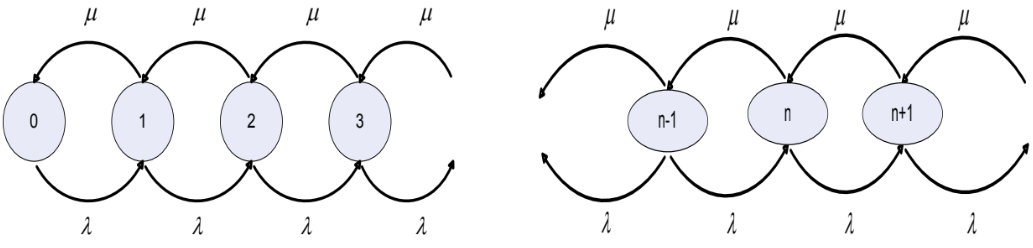
\includegraphics[width=4.5in]{chapters/chapter3/figures/Figura1-5:DiagramadeTransiciondeEstadosDTEdelsistema.png}
%%\centerline{\epsfig{/Chapters/chapter3/figures/Figura1-1:Sistema(mm1).png,width=.8\textheight,height=.4\textwidth}}
\caption[Diagrama de Transición de Estados DTE del sistema (M/M/1)]{Diagrama de Transición de Estados DTE del sistema (M/M/1)}
\label{fig:mesh5}
\end{figure}

De la misma manera como se estudió en la sección 1.3.1, en donde se trataron los sistemas de “nacimiento puro”, se empleará la misma notación para el proceso de nacimiento involucrado aquí. Las expresiones \ref{eqn:1.33}, \ref{eqn:1.34} y \ref{eqn:1.35} son el fundamento del proceso de nacimiento incluido en el proceso general de nacimiento y muerte.


\begin{equation}
   P \left [ Exactamente\; llegada\; en\;\left [ t,t+\Delta t \right ] \right ]=\lambda \Delta t
   \label{eqn:1.33}
\end{equation}



\begin{equation}
    P \left [ Ninguna\; llega\; en\;\left [ t,t+\Delta t \right ] \right ]=1-\lambda \Delta t
    \label{eqn:1.34}
\end{equation}



\begin{equation}
    P \left [ Mas\; de\; 1\; llegada\; en\; \left [ t,t+\Delta t \right ] \right ]=0
    \label{eqn:1.35}
\end{equation}
\\
También es necesario incorporar el proceso (de muerte) de acuerdo con el análisis de la sección 1.3.8. Las expresiones \ref{eqn:1.36}, \ref{eqn:1.37} y \ref{eqn:1.38} son el fundamento del proceso de muerte
incluido en el proceso general de nacimiento y muerte. 

\begin{equation}
   P \left [ Exactamente\; 1\; salida\; en\; \left [ t,t+\Delta t \right ] \right ]=\mu \Delta t
   \label{eqn:1.36}
\end{equation}

\begin{equation}
   P \left [ Ninguna\;  salida\; en\; \left [ t,t+\Delta t \right ] \right ]=1-\mu \Delta t
   \label{eqn:1.37}
\end{equation}

\begin{equation}
   P \left [ Mas\;  de\; 1\; salida\; en\; \left [ t,t+\Delta t \right ] \right ]=0
   \label{eqn:1.38}
\end{equation}
\\
El objetivo es encontrar $P_{n}\left ( t \right )$ , la función de densidad de la variable aleatoria $N_{t}$, es decir el estado del sistema, que denota el número de clientes dentro del sistema en el instante $t$ cuando la dinámica del sistema obedece a un proceso de nacimiento y muerte. Formalmente, la expresión \ref{eqn:1.39} define este concepto.

\begin{equation}
    f_{n_{t}}\left ( n \right )=P_{n}\left ( t \right )\equiv P\left [ N_{t}=n\; en\; el\; intervalo\; [0,t) \right ]
    \label{eqn:1.39}
\end{equation}
\\
Y sea $p_{ij}\left ( \Delta t \right )$ la probabilidad de pasar del estado (número de clientes dentro del sistema) $i$ al estado (número de clientes dentro del sistema) $j$ en un intervalo de tiempo de $\Delta t$ segundos.
\\
A partir de las expresiones numeradas desde la \ref{eqn:1.33} a la \ref{eqn:1.39} se deduce la expresión \ref{eqn:1.40}

\begin{equation}
    P_{n}\left ( t+\Delta t \right )
    = P_{n}\left ( t \right ) p_{n,n}\left ( \Delta t \right )+P_{n-1}\left ( t \right )p_{n-1,n}\left ( \Delta t \right )+P_{n+1}\left ( t \right )p_{n+1,n}\left ( \Delta t \right )
    \label{eqn:1.40}
\end{equation}
\\
Términos de orden superior funcionalmente dependientes de $\Delta t$ son ignorados puesto que son, en magnitud, muy pequeños. La ecuación \ref{eqn:1.40} dice que se puede llegar a tener $n$ clientes en el tiempo
$t+\Delta t$ ya sea porque el estado era $n-1$, $n$ ó $n+1$ clientes en el tiempo $t$. Debido a que se está frente a un proceso de $nacimiento$ $y$ $muerte$, estas son las únicas posibilidades. Para llegar al estado 0, se tendrá la condición inicial y, es evidente que, esa es una situación es especial y que se cumple la ecuación \ref{eqn:1.41}.

 \begin{equation}
     P_{0}(t+\Delta t)=P_{0}(t)p_{0,0}(\Delta t)+P_{1}(t)p_{1,0}(\Delta t)
     \label{eqn:1.41}
 \end{equation}
 \\
 Ahora sustituyendo en la expresión \ref{eqn:1.41} las probabilidades
 $p_{ij}(\Delta t)$ de acuerdo con las definiciones de nacimientos de las ecuaciones \ref{eqn:1.33}, \ref{eqn:1.34} y \ref{eqn:1.35} así como las 
definiciones para el proceso de muertes dadas en las ecuaciones \ref{eqn:1.36}, \ref{eqn:1.37} y \ref{eqn:1.38} para los eventos que ocurren en un intervalo $[t,t+\Delta t]$ , la expresión \ref{eqn:1.40} se convierte en la ecuación

\begin{equation}
    P_{n}(t+\Delta t)=P_{n}(t)(1-\Delta t)(1-\mu \Delta t)+P_{n-1}(t)(\lambda \Delta t)+P_{n+1}(t)(\mu \Delta t)
    \label{eqn:1.42}
\end{equation}
\\
Mientras que, bajo esas mismas consideraciones, la expresión \ref{eqn:1.41} se transforma en \ref{eqn:1.43}.

\begin{equation}
    P_{0}\left ( t+\Delta t \right ) = P_{0}\left ( t \right )\left ( 1-\lambda \Delta t \right )+P_{1}\left ( t \right )\left ( \mu \Delta t \right )
    \label{eqn:1.43}
\end{equation}
\\
Realizando unas sencillas operaciones algebraicas, reorganizando y tomando el límite cuando $ \Delta t \to 0 $ sobre las ecuaciones \ref{eqn:1.42} y \ref{eqn:1.43} se llega a la expresión \ref{eqn:1.44}

\begin{equation}
    \frac{dP_{n}\left ( t \right )}{dt}=-\left ( \lambda+\mu \right )P_{n}\left ( t \right )+\lambda P_{n-1}\left ( t \right )+\mu P_{n+1}\left ( t \right )
    \label{eqn:1.44}
\end{equation}
\\
Y a la ecuación \ref{eqn:1.45}.

\begin{equation}
    \frac{dP_{0}\left ( t \right )}{dt}=-\lambda P_{0}\left ( t \right )+\mu P_{1}\left ( t \right )
    \label{eqn:1.45}
\end{equation}
\\
Para $ n \geq 1 $.
\\


Las ecuaciones diferenciales \ref{eqn:1.44} y \ref{eqn:1.45}, describen la evolución de las probabilidades $P_{n}(t)$ de los estados del sistema de líneas de espera $(M/M/1)$ a través del tiempo. Pero ¿qué significan realmente estas ecuaciones? La respuesta a esta pregunta necesitará una discusión posterior sobre flujos y balances.
\\\\
Un caso muy útil e interesante sucede cuando $\frac{dP_{n}(t)}{dt}=0$; es decir cuando la estructura de probabilidades no cambia en función del tiempo. Esta es la situación que ocurre cuando el sistema de filas ha estado operando por mucho tiempo, el comportamiento se ha estabilizado transitoriamente y en la que el sistema ha llegado a un punto de equilibrio. Por ese motivo se dice que el sistema está en $equilibrio$ o $en$ $estado$ $estable$.
\\\\
En este caso, al ser la derivada igual a cero, las probabilidades asociadas con el estado del sistema no cambiarán (serán constantes) y, en consecuencia, no dependerán del tiempo $t$. Por esa razón no
es necesario escribirlas como funcione $P_{n}\left ( t \right )$ sino como constantes $ p_{n} $. De esta manera, las
ecuaciones diferenciales \ref{eqn:1.44} y \ref{eqn:1.45} se convierten en las expresiones \ref{eqn:1.46} y \ref{eqn:1.47}
respectivamente.

\begin{equation}
    0 = - \left ( \lambda + \mu \right )p_{n}+ \lambda p_{n-1} + \mu p_{n+1}
    \label{eqn:1.46}
\end{equation}

\begin{equation}
    0 = - \lambda p_{0}+\mu p_{1}
    \label{eqn:1.47}
\end{equation}
Para $ n \geq 1 $.
\\

Las ecuaciones resultantes son un conjunto de ecuaciones lineales en lugar de un conjunto de ecuaciones diferenciales, lo cual simplifica su solución. Para calcular las probabilidades de equilibrio, $p_{n} n=0,1,2,\cdots,N$, que gobiernan los estados de cualquier sistema de filas con un número $N$1 finito de estados, se procede de la siguiente manera. Para cada uno de los $N$1 estados se escribe una ecuación global de balance. Esto da un sistema de $N$+1 ecuaciones lineales con $N$+1 incógnitas. Ninguna de estas ecuaciones es redundante y, adicionalmente, debe ser incluida la ecuación \ref{eqn:1.48} para normalizar la solución y, al mismo tiempo, garantizar que el conjunto de todas las probabilidades encontradas constituyan una densidad de probabilidad.

\begin{equation}
    p_{0}+p_{1}+p_{2}+ \cdots + p_{N}=1 
    \label{eqn:1.48}
\end{equation}
\\
La solución del conjunto de ecuaciones lineales puede ser solucionado utilizando técnicas numéricas estándar. La razón por la cual es indispensable obtener todas las probabilidades a partir de ellas (y no antes) es posible determinar las medidas de desempeño, descritas en la sección 1.2.2, para cualquier sistema de líneas de espera.
\\

La dificultad que tiene esta aproximación es que en los modelos de colas reales frecuentemente el número de posibles estados del sistema es extremadamente grande haciendo la solución computacional casi imposible. Por suerte, en esos casos se puede suponer un sistema con capacidad infinita (en la práctica número de estados muy grande) y aplicar para esa situación un resultado matemático de extrema utilidad y belleza. Supóngase que se redibuja el diagrama de Transición de Estados, $DTE$ , del sistema $ \left ( M/M/1 \right ) $ como en la Figura \ref{fig:mesh6}.


\begin{figure}[H]
\centering
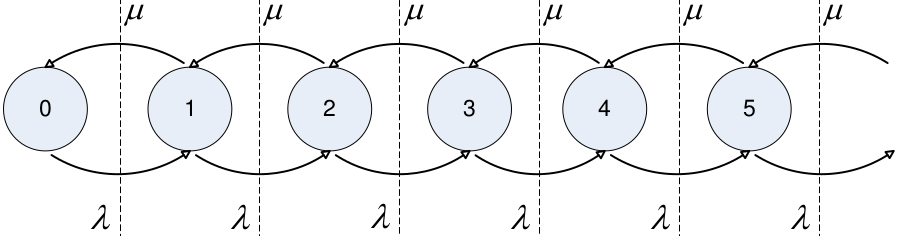
\includegraphics[width=4.5in]{chapters/chapter3/figures/Figura1-6:Balancelocalenlafronteraentreestados.png}
%%\centerline{\epsfig{/Chapters/chapter3/figures/Figura1-1:Sistema(mm1).png,width=.8\textheight,height=.4\textwidth}}
\caption[Balance local en la frontera entre estados]{Balance local en la frontera entre estados}
\label{fig:mesh6}
\end{figure}    

En ese $DTE$ se marcan con líneas punteadas verticales las fronteras entre cada par adyacente de estados. Cada frontera separa el diagrama de estado de transición en dos mitades. Es posible
equiparar el flujo de izquierda a derecha a través de tal frontera con el flujo de derecha a izquierda. Así se obtiene un conjunto de {\em ecuaciones locales de balance}. De cada una de esas fronteras
imaginarias surge una ecuación cuyo patrón se presenta en la expresión \ref{eqn:1.49}.

\begin{equation}
    \lambda p_{n-1}=\mu p_{n}
    \label{eqn:1.49}
\end{equation}
\\
Para $ n=1,2,3,\cdots $ (hasta infinito puesto que se empezó suponiendo un sistema con infinitos estados). Y, de ahí, fácilmente se deduce la ecuación \ref{eqn:1.50}.

\begin{equation}
    p_{n}=\frac{\lambda}{\mu}p_{n-1}
    \label{eqn:1.50}
\end{equation}
\\
Ahora, a través de un sencillo procedimiento recursivo, que se detiene para $ n=1 $, es fácil verificar que la solución de la ecuación en diferencias \ref{eqn:1.50} es \ref{eqn:1.51}.

\begin{equation}
    p_{n}\left ( \frac{\lambda}{\mu} \right )^{2}p_{0}
    \label{eqn:1.51}
\end{equation}
\\
Finalmente, puesto que $ \displaystyle\sum_{n=0}^{+\infty }p_{n}=\sum_{n=0}^{+\infty }\left ( \frac{\lambda}{\mu} \right )^{n}p_{0}=1 $, por ser una función de densidad de probabilidad discreta, se obtiene la probabilidad de que el sistema esté desocupado \ref{eqn:1.52}.

\begin{equation}
    p_{0}=\frac{1}{\displaystyle\sum_{n=0}^{+\infty }\left ( \frac{\lambda}{\mu} \right )^{n}}
    \label{eqn:1.52}
\end{equation}
\\
\section{EL SISTEMA DE FILAS \textit{(M/M/1)} EN DETALLE}
\subsection{Función de densidad}
Es posible simplificar la expresión \ref{eqn:1.52} para calcular p 0 al emplear la “serie geométrica” dada en la identidad \ref{eqn:1.53} con $ \rho = \frac{\lambda}{\mu} $. Para que esa identidad pueda ser empleada es necesario imponer la restricción $ \lambda < \mu $.

\begin{equation}
    \sum_{n=0}^{\infty }\rho=\frac{1}{1-\rho} \; con\;\; 0\leq \rho< 1
    \label{eqn:1.53}
\end{equation}
\\
De esta manera, entonces,$ p_{0}= \left ( 1-\rho \right ) $ y, en consecuencia, la función de densidad sobre los estados del sistema se obtiene a partir de \ref{eqn:1.51} y se presenta en la ecuación \ref{eqn:1.54}.

\begin{equation}
    p_{n}=\left ( 1-\rho \right )\rho_{n}
    \label{eqn:1.54}
\end{equation}
\\
\subsection{Utilización del servidor}
La probabilidad de que el servidor esté ocupado (es decir que no esté libre) se denomina “la utilización del servidor”. Esta probabilidad se interpreta como el porcentaje del tiempo de operación del sistema en el cual el servidor estuvo ocupado atendiendo a los clientes del sistema. Formalmente esta medida de desempeño se calcula como se muestra en la ecuación \ref{eqn:1.55}.

\begin{equation}
    U=P\left [ N_{t}> 0 \right ]=1-P\left [ N_{t}=0 \right ]=1-p_{0}=\rho
    \label{eqn:1.55}
\end{equation}
\\
En consecuencia el parámetro $ \rho = \frac{\lambda}{\mu} $ se conoce como {\em utilización}. La magnitud $ \rho $ puede verse como la \textbf{\textit{carga ofrecida}} normalizada. Esto es, $ \lambda $ puede variar desde cero (carga suave), hasta un valor ligeramente menor que $ \mu $ (carga pesada). Además, $ \rho $ puede variar entre 0 y 1. \\


Aunque para llegar a esta conclusión se supuso que la capacidad del sistema es infinito, en la práctica, sin embargo, las probabilidades de que en el sistema hayan muchos clientes esperando a ser atendidos es relativamente pequeña y depende, obviamente, de la “carga ofrecida” por el sistema.

\subsection{Número medio de clientes en el sistema}
El número medio $ \mu_{N_{t}} $ de clientes que se encuentran en el sistema está dado en la ecuación \ref{eqn:1.56}.
\begin{equation}
    \mu_{N_{t}}=E\left [ N_{t} \right ]=\frac{\rho}{1-\rho}
    \label{eqn:1.56}
\end{equation}
\\
Para mostrar que \ref{eqn:1.56} es cierta, considérense los dos comentarios que siguen:

\begin{enumerate}
    \item $\displaystyle\sum_{n=0}^{\infty }n\rho^{n}=\rho\sum_{n=1}^{\infty }n\rho^{n-1}=\rho\frac{d}{d\rho}\left ( \frac{1}{1-\rho} \right )=\frac{\rho}{\left ( 1-\rho \right )^{2}} $. Es decir que $ \displaystyle\sum_{n=0}^{\infty }n\rho^{n}=\frac{\rho}{\left ( 1-\rho \right )^{2}} $. Este resultado se empleará en uno de los pasos del numeral 2 que sigue.
    \item $ \mu_{N_{t}}=E\left [ N_{t} \right ]=\displaystyle\sum_{n=0}^{\infty }n\rho_{n}=\sum_{n=0}^{\infty }n\left ( 1-\rho \right )\rho^{n}=\left ( 1-\rho \right )\sum_{n=0}^{\infty }n\rho^{n}= \left ( 1-\rho \right )\left [ \frac{\rho}{\left ( 1-\rho \right )^{2}} \right ]=\frac{\rho}{\left ( 1-\rho \right )} $.
\end{enumerate}

La función descrita por la ecuación ( \ref{eqn:1.56} se presenta en la Figura \ref{fig:mesh7}. Lo que es más notable de esta función es un incremento no lineal asintótico en el número medio de clientes en el sistema conforme $ \rho \to 1 $. También es interesante comentar que esta función se utiliza con frecuencia como una “función de penalización” en optimización de algoritmos en filas largas de espera.

\begin{figure}[H]
\centering
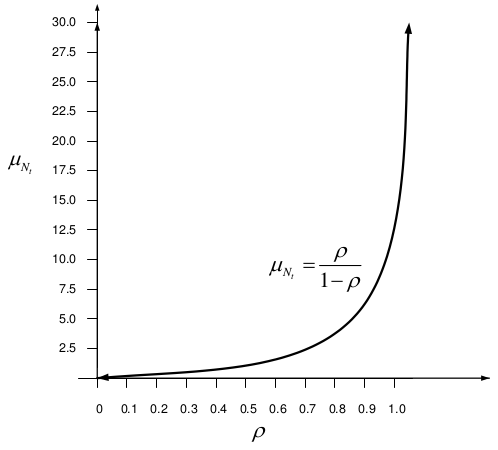
\includegraphics[width=3in]{chapters/chapter3/figures/Figura1-7:Numeromediodeclientesenunsistema.png}
%%\centerline{\epsfig{/Chapters/chapter3/figures/Figura1-1:Sistema(mm1).png,width=.8\textheight,height=.4\textwidth}}
\caption[Número medio de $ \mu_{N_{t}} $ clientes en un sistema (M/M/1)]{Número medio de $ \mu_{N_{t}} $ clientes en un sistema (M/M/1)}
\label{fig:mesh7}
\end{figure}    

\subsection{Varianza del Número de clientes en el sistema.}

LA varianza $ \sigma_{N_{t}}^{2} $ del número de clientes que se encuentran en el sistema está dada en la ecuación \ref{eqn:1.57}. 

\begin{equation}
    \sigma_{N_{t}}^{2}=E\left [ \left ( N_{t}-\mu _{N_{t}} \right )_{t}^{2} \right ]=\frac{\rho}{\left ( 1- \rho \right )^{2}}
    \label{eqn:1.57}
\end{equation}
\\
Para mostrar que \ref{eqn:1.56} es cierta, considérense los dos comentarios que siguen:

\begin{enumerate}
    \item $ \sigma_{N_{t}}^{2}=E\left [ \left ( N_{t}-\mu _{N_{t}} \right )_{t}^{2} \right ]= E\left [ N_{t}^{2} \right ]-\left ( \mu _{N_{t}} \right )^{2} $. Nótese que $ \mu _{N_{t}} $ está dada en la expresión \ref{eqn:1.56} y, por lo tanto, es suficiente con calcular el segundo momento del número de clientes en el sistema $ N_{t} $
    \item Antes de ello es fácil verificar que $ \displaystyle\sum_{n=0}^{\infty }n^{2}\rho^{n}=\frac{\rho \left ( 1+\rho \right )}{\left ( 1-\rho \right )^{3}} $. Este resultado se empleará en uno de los pasos del numeral 3 que sigue.
    \item $ E\left [ N_{t}^{2} \right ] = \displaystyle\sum_{n=0}^{\infty }n^{2}\rho_{n}= \sum_{n=0}^{\infty }n^{2}\left ( 1- \rho \right )\rho^{n}= \left ( 1- \rho \right )\frac{\rho \left ( 1+\rho \right )}{\left ( 1-\rho \right )^{3}}=\frac{\rho \left ( 1+\rho \right )}{\left ( 1-\rho \right )^{2}} $. Finalmente, reemplazando este resultado en el comentario 1, se sigue el resultado. 
\end{enumerate}

El comportamiento de la variabilidad del número de clientes en el sistema se presenta en la Figura
\ref{fig:mesh8}. Al igual que con el número

\begin{figure}[H]
\centering
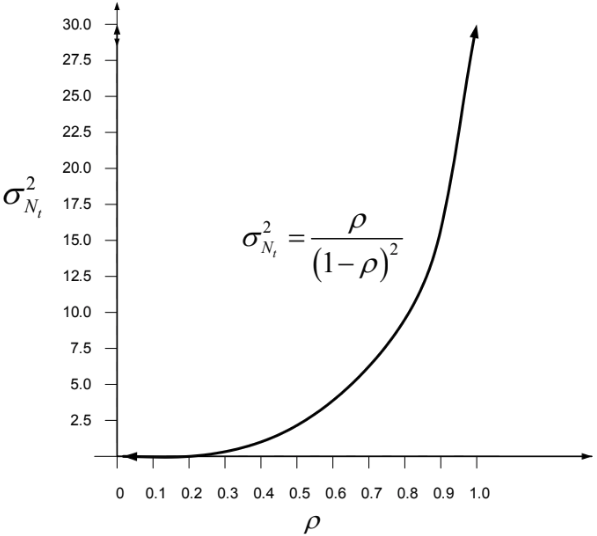
\includegraphics[width=3in]{chapters/chapter3/figures/Figura1-8:Varianzadelnumerodeclientesenunsistema.png}
%%\centerline{\epsfig{/Chapters/chapter3/figures/Figura1-1:Sistema(mm1).png,width=.8\textheight,height=.4\textwidth}}
\caption[Varianza del número de clientes $ \sigma_{N_{t}}^{2} $ en un sistema (M/M/1)]{Varianza del número de clientes $ \sigma_{N_{t}}^{2} $ en un sistema (M/M/1)}
\label{fig:mesh8}
\end{figure} 

\section{LEY DE LITTLE}
La ley de Little es el resultado teórico que permite calcular otra medida de desempeño importante en sistemas de línea de espera: {\em El Tiempo medio que un cliente permanece dentro del sistema. } Formalmente, sea $ T $ la variable aleatoria que representa el tiempo que un cliente “gasta” desde el momento de su llegada al sistema hasta el momento en el cual el servidor termina de atenderlo. De
acuerdo con lo discutido en la sección 1.2.2, entonces, se desea encontrar $ \mu_{T} = E \left[ T \right] $. Una forma de encontrar ésta constante es realizar el cálculo aplicando directamente la definición de esperanza matemática; sin embargo, para ello es necesario contar con $ f_{T}\left( t \right) $, información con la cual no se cuenta.
\\
Una forma alternativa, más directa, simple, eficiente y elegante, es emplear la ecuación llamada la “Ley de Little” \footnote{La notación original empleada por Little para esta ley es $ L=\lambda W. $}

\begin{equation}
    \mu_{N} = \lambda \mu_{T}
    \label{eqn:1.58}
\end{equation}
\\
Nótese que $ \lambda $ es la tasa de llegadas de clientes al sistema de líneas de espera. Así mismo, se cuenta $ \mu_{N_{t}} $ al aplicar la ecuación \ref{eqn:1.56}, en consecuencia, $ \mu_{T} $ se puede deducir fácilmente a partir de \ref{eqn:1.58}.

En \cite{kleinrock1975} se presentan al menos cinco demostraciones diferentes de este interesante y útil resultado\footnote{La ley de Little también se tiene si consideramos la fila y no el servidor, 
esto es $ \mu_{N}^{\left ( Q \right )}=\lambda \mu_{T}^{\left ( Q \right )}. $}. El esquema de demostración que aquí se presenta está inspirado en una de esas pruebas. La Figura\ref{fig:mesh9} ayuda a entender ésta estrategia de demostración.

\begin{figure}[H]
\centering
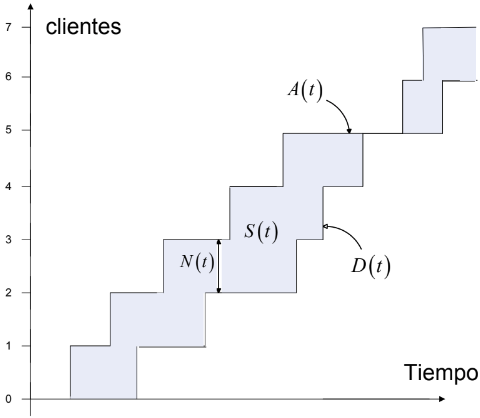
\includegraphics[width=2.5in]{chapters/chapter3/figures/Figura1-9:EsquemadedemostraciondelaLeydeLittle.png}
%%\centerline{\epsfig{/Chapters/chapter3/figures/Figura1-1:Sistema(mm1).png,width=.8\textheight,height=.4\textwidth}}
\caption[Esquema de demostración de la ``Ley de Little'']{Esquema de demostración de la ``Ley de Little''}
\label{fig:mesh9}
\end{figure} 

Las bases de la prueba se enumeran a continuación:

\begin{enumerate}
    \item Considerando el intervalo de tiempo $ \left [ 0,t \right] $ y sean las funciones: $ A \left ( t \right) $ que denota el número de llegadas al sistema hasta el instante $ t $. $ D\left ( t \right) $ que representa el número de salidas del sistema hasta el instante $ t $. Por esta razón $ N\left ( t \right) = A\left ( t \right)-D\left ( t \right) $ será el número de clientes en el sistema en el instante $ t $. 
    \item $ S\left ( t \right) $ es el área acumulada entre las curvas $ A\left ( t \right) $ y $ D\left ( t \right) $ hasta el tiempo $ t $. Esta área es el tiempo total utilizado por todos los clientes que han estado en el sistema hasta el instante $ t $. 
    \item Con ello, ahora, se formalizan tres relaciones evidentes en la Figura \ref{fig:mesh9}.
    \begin{enumerate}
        \item La primera es $ \lambda_{t} = \frac{A\left ( t \right)}{t} $. Aquí, $ \lambda_{t} $ es la tasa media de llegadas durante el $\left [ 0,t \right]$.
        \item La segunda es $ \mu_{T}^{\left ( t \right)} = \frac{S\left ( t \right)}{A\left ( t \right)} $ el tiempo medio que han empleado los cliente en el hasta el instante $ t $.
        \item Y, por último, la tercera ecuación es $ \mu_{N}^{\left ( t \right)} = \frac{S\left ( t \right)}{t} $ el número promedio de clientes hasta el instante $ t $.
    \end{enumerate}
    \item De ahí, es claro que $ \mu_{N}^{\left ( t \right)} = \frac{S\left ( t \right)}{t} = \frac{\mu_{T}^{\left ( t \right)}\times A\left ( t \right) } {t} = \lambda_{t} \times \mu_{T}^{\left ( t \right)} $. Es decir, $ \mu_{N}^{\left ( t \right)} = \lambda_{t} \times \mu_{N}^{\left ( t \right)} $. 
    \item Finalmente, tomando el límite cuando $ t \to \infty $ , $ \mu _{N} =\lim_{t\to 0} \left ( \mu_{N}^{\left( t \right) } \right ) $, $ \lambda \lim_{t\to 0} \left( \lambda_{t} \right)$ y $ \mu _{T} =\lim_{t\to 0} \left ( \mu_{T}^{\left( t \right) } \right ) $, De donde se concluye la ley $ \mu_{N}= \lambda \mu_{T} $.
\end{enumerate}

La ley de Little aplica, en general, para cualquier sistema de líneas de esperas $ \left ( G/G/m \right ) $ y en particular para los sistemas $ \left ( M/M/1 \right ) $, como se muestra en el ejemplo que sigue.
\\
\\
\textbf{Ejemplo 1—3}
El cálculo de $ \mu _{T} $ para el sistema $ \left ( M/M/1 \right ) $ a partir de la “Ley de Little” mostrada en la ecuación \ref{eqn:1.58}, puede realizarse usando el resultado de la ecuación \ref{eqn:1.56}, por lo tanto $  $



\section{TEOREMA DE BURKE}
\begin{theorem}[Teorema de Burke]\label{1th:Z_m}
El proceso de salida de un proceso para un sistema $ \left( M/M/1 \right) $, en equilibrio, es un proceso de Poisson con parámetro $ \lambda $.
\end{theorem}

\section{RESUMEN Y PANORAMA HISTÓRICO}
En este capítulo se estudió la teoría de colas simple, una de las ramas de la investigación de operaciones. El estudio matemático de las filas que se forman en ciertos sistemas es fundamental para optimizar la operación del sistema. Por esta razón, el principal propósito de esta disciplina es caracterizar dicho sistema desde el punto de vista de su rendimiento. Medidas de desempeño tales
como el tiempo de espera medio en las colas o la utilización del sistema para que éste mantenga su normal operación sin que llegue a colapsar o, al menos, conocer las circunstancias que producirían tal situación.
\\
\\
Su aplicabilidad a las ciencias de la computación, las redes de computadores y las telecomunicaciones es evidente. En este sentido, la teoría es muy útil para modelar procesos tales como la llegada de datos a una cola en ciencias de la computación, la congestión de redes de computadores, redes Ad Hoc, sistemas celulares y, en general, redes de telecomunicaciones. Otras aplicaciones en el contexto de la computación son también evidentes. Por ejemplo, los procesos enviados a un servidor para su ejecución forman colas de espera mientras no son atendidos; la información solicitada, a través de Internet, a un servidor Web puede recibirse con demora debido a la congestión en la red. 
\\
\\
El origen de esta teoría se encuentra en los estudios del matemático, estadístico, e ingeniero danés Agner Krarup Erlang quien nació en el año de 1878 y murió en 1929. A él se le da el apelativo de “Padre de la Ingeniería de Teletráfico” puesto que en 1909, para analizar la congestión del tráfico telefónico con el propósito de satisfacer adecuadamente la demanda estocástica de servicios en el sistema telefónico de Copenhague, empezó por formalizar o matematizar el comportamiento de estos sistemas.


\section{EJERCICIOS}

\begin{enumerate}
    \item Dado el sistema de colas determinístico, tanto en su proceso de llegadas como en el de servicio, $ \left ( \lambda / \mu / 1 \right ) $ con tasas de llegadas y de atención $ \lambda, \mu \in \mathbb{R}^{+} $ respectivamente cuyas unidades son $ \displaystyle paquetes / segundo $ . Deduzca formalmente las siguiente medidas de desempeño (Imponga las restricciones y proponga los supuestos que sean necesarios):
    \begin{enumerate}
        \item Utilización.
        \item Número medio de clientes en fila.
        \item Número medio de clientes en el sistema.
        \item Tiempo medio en fila.
        \item Tiempo medio en el sistema.
    \end{enumerate}
    \item Para un proceso binomial con $ \lambda = 5 clientes/Seg  t=10 seg $ y $ \delta t = 0.1 $, encuentre:
    \begin{enumerate}
        \item La función de densidad.
        \item La función percentil.
        \item La varianza.
        \item La función generadora de momentos.
        \item La probabilidad de que después de los primeros $ 5seg $ no lleguen clientes.
    \end{enumerate}
    \item En la sección 1.3.3 se dedujo el modelo de nacimiento puro. Haciendo un desarrollo similar, formule los fundamentos de un proceso de muerte pura.
    \item * Demuestre que, en el caso continuo, la familia exponencial $ T \sim Exp \left ( \lambda \right ) $ es la ÚNICA familia que exhibe la propiedad de pérdida de la memoria.
    \item Con un procedimiento análogo (esto es similar) al empleado en la sección 1.3.6 para demostrar que la familia exponencial presenta la propiedad de pérdida de la memoria, 
    \begin{enumerate}
        \item Demuestre que, en el caso discreto, la familia Geométrica $ T \sim Geo \left ( p \right ) $ presenta la propiedad de pérdida de la memoria.
        \item * Demuestre que, en el caso discreto, la familia Geométrica $ T \sim Geo \left ( p \right ) $ es la ÚNICA familia que exhibe la propiedad de pérdida de la memoria.
    \end{enumerate}
\end{enumerate}
